% \section{MMORE Performances \& Applications}
\section{Results}

\subsection{Processing}


% %%% Acc. table
\begin{table*}[t]
\centering
\small
\resizebox{0.72\textwidth}{!}{%
\begin{tabular}{lcccccc}
\toprule
 & \multicolumn{3}{c}{\textit{The Blue Castle (digital PDF)}} & \multicolumn{3}{c}{\textit{The Great Gatsby (scanned images)}} \\
\cmidrule(lr){2-4} \cmidrule(lr){5-7}
Method & BLEU\textbf{$\uparrow$} & ROUGE-L\textbf{$\uparrow$} & CER\textbf{$\downarrow$} & BLEU\textbf{$\uparrow$} & ROUGE-L\textbf{$\uparrow$} & CER\textbf{$\downarrow$} \\ 
\midrule
\rowcolor{orange!10}
MMORE &0.8608 & 0.9940 & 0.0241 & \textbf{0.7973} & \textbf{0.9813} & \textbf{0.0295} \\
MMORE (fast)    & 0.8639 & \textbf{0.9963} & 0.0206 & 0.0000 & 0.0000 & 1.0000 \\
Docling         & \textbf{0.8643} & 0.9959 & \textbf{0.0199} & 0.5451 & 0.6582 & 0.5518 \\
\bottomrule
\end{tabular}%
}
\caption{Accuracy evaluation on two Project Gutenberg books: ``\textit{The Blue Castle}'' and ``\textit{The Great Gatsby}''.}
\label{tab:accuracy_results}
\end{table*}

%% Eff. figure
\begin{figure}[ht]
    \centering
    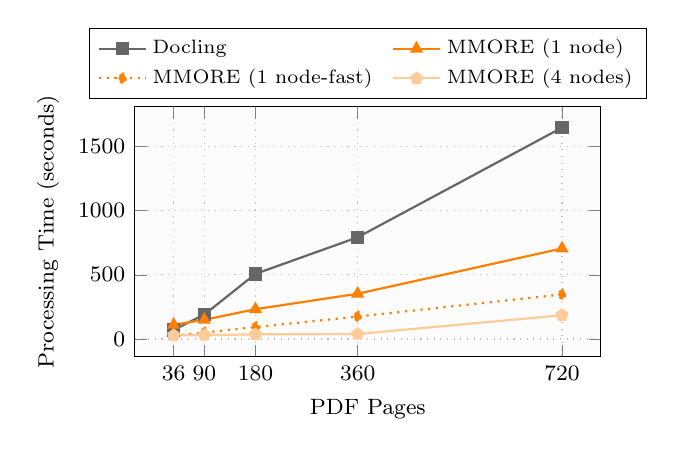
\begin{tikzpicture}
        \begin{axis}[
            xlabel={PDF Pages},
            ylabel={Processing Time (seconds)},
            legend style={
                font=\scriptsize,
                cells={anchor=west},
                at={(0.5,1.03)},
                anchor=south,
                legend columns=2,
                /tikz/every even column/.append style={column sep=0.5em}
            },
            grid=both,
            grid style={dotted,gray!50},
            xtick={36,90,180,360,720},
            width=7.5cm,
            height=4.75cm,
            scaled ticks=false,
            ticklabel style={/pgf/number format/1000 sep={}},
            label style={font=\footnotesize},
            tick label style={font=\footnotesize},
            every axis plot/.append style={thick},
            axis background/.style={fill=gray!2},
        ]

        % Docling (Black)
        % \addplot[color=black!50, mark=square*] table {
        %     36 70.66
        %     90 190.44
        %     180 507.23
        %     360 792.43
        %     720 1647.56
        % };
        % \addlegendentry{Docling}

        % Docling (Blue)
        \addplot[color=black!60, mark=square*] table {
            36 70.66
            90 190.44
            180 507.23
            360 792.43
            720 1647.56
        };
        \addlegendentry{Docling}
        
        % MMORE (1 node) - orange solid
        \addplot[color=orange, mark=triangle*, solid] table {
            36 110.67
            90 149.35
            180 232.05
            360 352.53
            720 705.33
        };
        \addlegendentry{MMORE (1 node)}

        % MMORE (1 node-fast) - orange dotted
        \addplot[color=orange, mark=diamond*, dotted] table {
            36 26.78
            90 50.29
            180 92.59
            360 174.66
            720 347.09
        };
        \addlegendentry{MMORE (1 node-fast)}

        % MMORE (4 nodes) - light orange solid
        \addplot[color=orange!40, mark=pentagon*, solid] table {
            36 28.19
            90 29.78
            180 35.71
            360 38.64
            720 185
        };
        \addlegendentry{MMORE (4 nodes)}

        \end{axis}
    \end{tikzpicture}
    \caption{Processing time vs. PDF length for \textit{Docling} and \mmore{}. \mmore{} (1 node-fast) disables OCR for performance, and \mmore{} (4 nodes) uses distributed processing.}
    \label{fig:pdf_processing}
\end{figure}

\textbf{Efficiency.} Figure~\ref{fig:pdf_processing} shows comparison of \textit{Docling} and \mmore{}. On short documents (36 pages) \textit{Docling} is marginally faster than \mmore{} (default). The difference disappears at 90 pages and shifts in favor of \mmore{} beyond 180 pages, where our pipeline scales almost linearly while \textit{Docling} slows down super-linearly. The fast mode, which omits OCR, delivers an additional speed-up of roughly two to three times. Running the default pipeline on four nodes achieves a 3.8-fold reduction in latency compared to the single-node baseline, surpassing even the single-node fast mode and clearly demonstrating the efficiency and scalability of the distributed execution in \mmore{}. It is also worth mentioning that the batch size is user-configurable. The experiments presented here used a conservative default, leaving around 65GB of the 80GB GPU unused. This highlights the potential for further optimization, as users can adjust the configuration to fully exploit available hardware resources. Table~\ref{tab:general_performance} further illustrates the performance advantage of \mmore{} across multiple file types. In default mode, \mmore{} reduces the total processing time by 45.48\% compared to \textit{Docling}, with the fast mode achieving an even more pronounced improvement of 155.38\%.

\begin{table}[ht]
\centering
\resizebox{0.46\textwidth}{!}} & \textcolor{green1!90!black}{\textbf{+155.38\%}} \\
\bottomrule
\end{tabular}%
}
\caption{Processing speeds for 9 unique file types - PDF, DOCX, EML, MD, MP4, MP3, PPTX, TXT, XLSX (19 files in total).}
\label{tab:general_performance}
\end{table}
\vspace{-0.2cm}

\textbf{Accuracy.} Table \ref{tab:accuracy_results} reports BLEU, ROUGE-L, and CER on two Project Gutenberg titles. On the digitally formatted "Blue Castle" book, all three systems achieve near-perfect scores, with \textit{Docling} attaining the lowest CER (1.99\%); however, differences remain negligible. The scanned version of "The Great Gatsby", an image-based document requiring OCR, provides a greater challenge. Here, \mmore{} fast predictably fails, as it omits OCR entirely. In contrast, \mmore{} default maintains high extraction fidelity, clearly outperforming \textit{Docling}, whose CER of 55\% indicates significant OCR errors. Although these results demonstrate the accuracy of our pipeline, further benchmarking on a larger and more diverse set of documents is necessary to robustly validate its generalization capabilities.

\subsection{RAG}

% \begin{table}[ht]
% \centering
% \begin{tabular}{@{}llcc@{}}
% \toprule
% \textbf{LLM} & \textbf{Mode} & \textbf{Retriever} & \textbf{PubMedQA} \\ 
%              &              &                     & $\pm$ 0.0193 \\ \midrule
% Meditron3-8B & No RAG & - & 0.754 \\ 
%              & With RAG (k=1) & bge-large-en-v1.5 & \underline{0.79} \\ 
%              & With RAG (k=3) & bge-large-en-v1.5 & \textbf{0.80} \\ \midrule

% Meditron3-70B & No RAG & - & 0.802 \\ 
%               & With RAG (k=1) & bge-large-en-v1.5 & \underline{0.81} \\ 
%               & With RAG (k=3) & bge-large-en-v1.5 & \textbf{0.82} \\ 
% \bottomrule
% \end{tabular}
% \caption{Results demonstrating the effectiveness of RAG in improving LLM performance on PubMedQA.}
% \label{tab:results_pubmed}
% \end{table}

\begin{figure}[h]
\centering
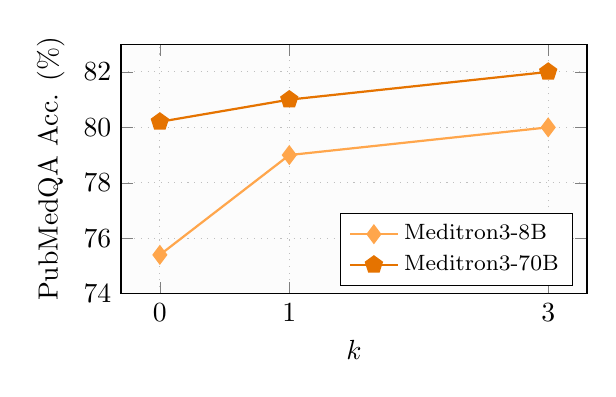
\begin{tikzpicture}
\begin{axis}[
    xlabel={$k$},
    ylabel={PubMedQA Acc. (\%)},
    xtick={0,1,3},
    ymin=74, ymax=83,
    legend pos=south east,
    grid=major,
    grid style={dotted,gray!50},
    width=7.5cm,
    height=4.75cm,
    mark size=3pt,
    scaled ticks=false,
    every axis plot/.append style={thick},
    axis background/.style={fill=gray!2},
    legend style={
            font=\footnotesize,
            cells={anchor=west},
        },
]

% Meditron3-8B line (orange shade, diamond marker)
\addplot[
    color=orange!70, 
    mark=diamond*
] coordinates {
    (0, 75.4)
    (1, 79.0)
    (3, 80.0)
};
\addlegendentry{Meditron3-8B}

% Meditron3-70B line (darker orange shade, pentagon marker)
\addplot[
    color=orange!90!black, mark=pentagon*
] coordinates {
    (0, 80.2)
    (1, 81.0)
    (3, 82.0)
};
\addlegendentry{Meditron3-70B}

\end{axis}
\end{tikzpicture}
\vspace{-0.3cm}
\caption{Effect of retrieved documents ($k$) on PubMedQA accuracy for Meditron models using \mmore{}'s built-in RAG.}
\label{fig:pubmedqa_rag}
\end{figure}
\vspace{-0.2cm}

To evaluate RAG performance, we test the Meditron-3 model family with various RAG configurations on the PubMedQA benchmark. Figure~\ref{fig:pubmedqa_rag} shows that both Meditron-3[8B] and Meditron-3[70B]~\cite{sallinen2025llama} consistently improve accuracy with RAG, especially as the number of retrieved documents $k$ increases. These results demonstrate that our RAG pipeline effectively injects domain-specific context at inference time, improving answer accuracy.

% RAG INFERENCE SPEED => GRAPH DB SIZE AS X, SPEED AS Y

% This demonstrate the effectiveness of using our RAG pipeline for enhancing the knowledge and performance of large language models (LLMs) in specialized domains, as exemplified by the PubMedQA benchmark. Our RAG system retrieves information from a vector database containing all PubMed abstracts and conclusions, ensuring access to relevant and high-quality context. Both Meditron3-8B and Meditron3-70B models \cite{meditron} show consistent improvements in accuracy when RAG is applied, particularly in settings where multiple retrieved documents are utilized. For instance, Meditron3-8B achieves a baseline accuracy of 0.7540 without RAG, which increases to 0.7900 with RAG using a single document and further improves to 0.8000 when three documents are retrieved. Similarly, Meditron3-70B exhibits a baseline accuracy of 0.8020, rising to 0.8100 with one document and reaching 0.8200 with three documents. These results highlight that our RAG pipeline not only retrieves the most relevant biomedical information effectively but also enables the LLM to leverage this context to improve its reasoning and accuracy. This confirms that our carefully designed RAG pipeline is highly effective when used in the right setting to maximize performance gains.